%!TEX root = main.tex
    We split a given population of size $N$ in the basic SEIR
structure with segregated classes according to the manifestation
of symptoms. Let $L, S, E, I_S, I_A, H, R, D$ respectively denote the
class of individuals according to their current state, namely
%
\begin{description}[%
    labelwidth=\widthof{\textbf{Infected-Asymptomatic $(I_A)$}},
    leftmargin=\widthof{\textbf{Infected-Asymptomatic $(I_A)$}},
    align=right%
]
    \item[Lockdown $(L)$:]
        All individuals that have low or null mobility and remain under
        isolation. Thus individuals in this class reduce their contagion 
        probability.
    \item[Susceptible $(S)$:]
        Individuals under risk.
    \item[Exposed $(E)$:]
        Population fraction that hosts SARS-CoV-2 but cannot infect.
    \item[Infected-Symptomatic $(I_S)$:]
        Population infected fraction with symptoms and reported as confirmed
        cases.
    \item[Infected-Asymptomatic $(I_A)$:]
        Infected individuals with transitory or null symptoms and unreported.
    \item[Hospitalized $(H)$:]
        Infected population that requires hospitalization or intensive care.
    \item[Recover or removed $(R)$:]
        Population that recovers from infection and develops partial immunity.
    \item[Death $(D)$:]
        Population fraction that died due to COVID-19.
\end{description}
%
To fit data of cumulative reported symptomatic cases, we
postulate the counter state $Y_{I_S}$ and make the following assumptions.
%
%
\begin{assumptions}
    According to above compartment description, we made the following
    hypotheses.
    \begin{enumerate}[label={(A-\arabic*)}]
        \item
            We suppose that at least \SI{30}{\percent} of the population is
            locked down and a fraction of this class eventually moves
            to the susceptible compartment at rate $\delta_L$.
        \item
            Force infection is defined as the probability of acquiring COVID-19
            given the contact with a symptomatic or asymptomatic individual.
            Thus we normalize with respect to alive population population
            $
                N^{\star}
            $.
        \item
            Susceptible individuals become
            exposed\textemdash but not infectious\textemdash
            % exposed individuals
            %host the virus but can not transmit it.
            when they are in contact with asymptomatic or symptomatic
            individuals. Thus $\beta_S$ and $\beta_A$ denote the
            probabilities of being infectious given the contact with a 
            symptomatic orasymptomatic infectious individuals, respectively.
        \item
            After a period of latency  $1/\kappa = \SI{5.1}{days}$, an
            exposed individual becomes infected. Being $p$ the probability of
            developing symptoms and $(1-p)$ the probability of becoming infectious
            but asymptomatic. Thus $p\kappa E$ denotes the
            exposed individuals that become infectious and develop symptoms.
        \item
            Asymptomatic individuals do not die or stay in the hospital.
        \item
            A fraction $\mu_{H}$ of symptomatic individuals
            dies due to COVID-19 without hospitalization.
        %\item
    \end{enumerate}
\end{assumptions}

\begin{figure*}[tbh]
    \centering
      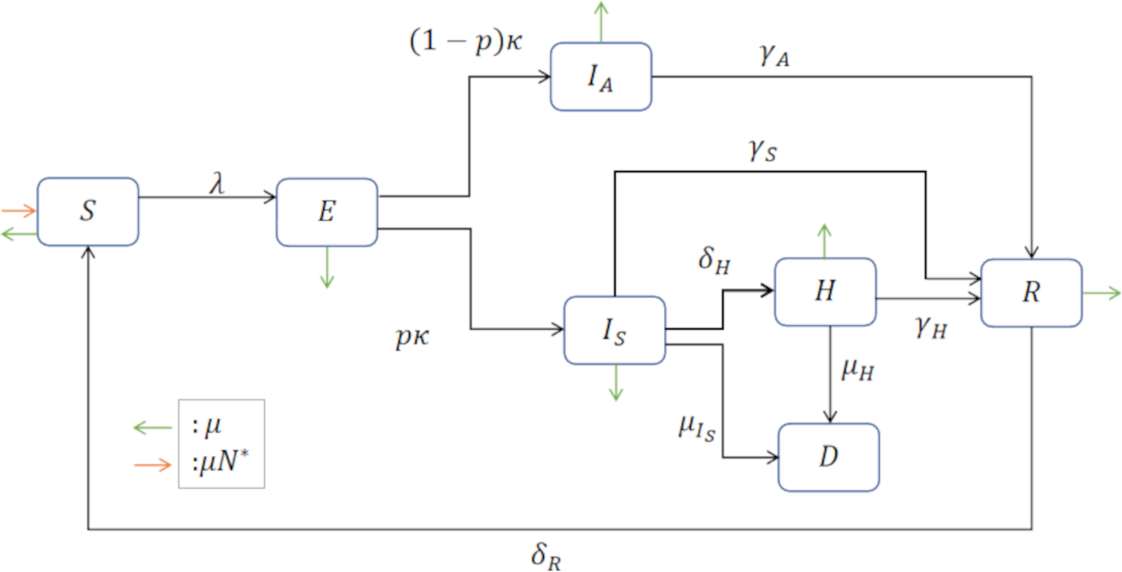
\includegraphics[scale=0.7, keepaspectratio]{Diagram_no_Vaccination.pdf}
        \caption{
            Compartmental diagram of COVID-19 transmission dynamics. 
            Consider the class: Susceptible $(S)$, exposed $(E)$, symptomatic 
            infected $(I_S)$, asymptomatic infected $(I_A)$, recovered $(R)$, 
            death $(D)$ and vaccinated $(V)$ individuals. It is important to 
            mention that $I_{S}$ represents the proportion of symptomatic 
            individuals who will later report to some health medical center.
        }
    \label{fig:diagramnolockdownandVacc}
\end{figure*}

Thus we formulate the following Ordinary Differential Equation (ODE), see
\Cref{fig:diagramnolockdownandVacc}, to complete the underlying description.
\begin{equation}
	\label{eqn:base_dynamics}
    \begin{aligned}
        S' & =
            \mu N^\star + \delta_R R - (\lambda + \mu)
            S,
        \\
        E' & =
            \lambda (\epsilon L + S) - (\kappa + \mu) E,
        \\
        I_S' & =
            p \kappa E -
            (\gamma_S +
                \delta_H +
                \mu_{I_S} +
                \mu) I_S,
        \\
        I_A' &=
            (1 - p) \kappa E - (\gamma_A + \mu) I_A,
        \\
        H' &=
            \delta_H I_S - (\gamma_H + \mu_H + \mu) H,
        \\
        R' & =
            \gamma_S I_S + \gamma_A I_A + \gamma_H H - (\delta_R + \mu) R,
        \\
        D' &=
            \mu_{I_S} I_S + \mu_H H,
        \\
        \frac{dY_{I_S}}{dt} &  = p \kappa E,
        \\
        \lambda &:=
            \frac{\beta_A I_A + \beta_S I_S}{N^{\star}},
        \\
        N^{\star}(t) &=
            L + S + E +
            I_S + I_A +
            H + R .
    \end{aligned}
\end{equation}
%
\begin{figure}
    \begin{center}
        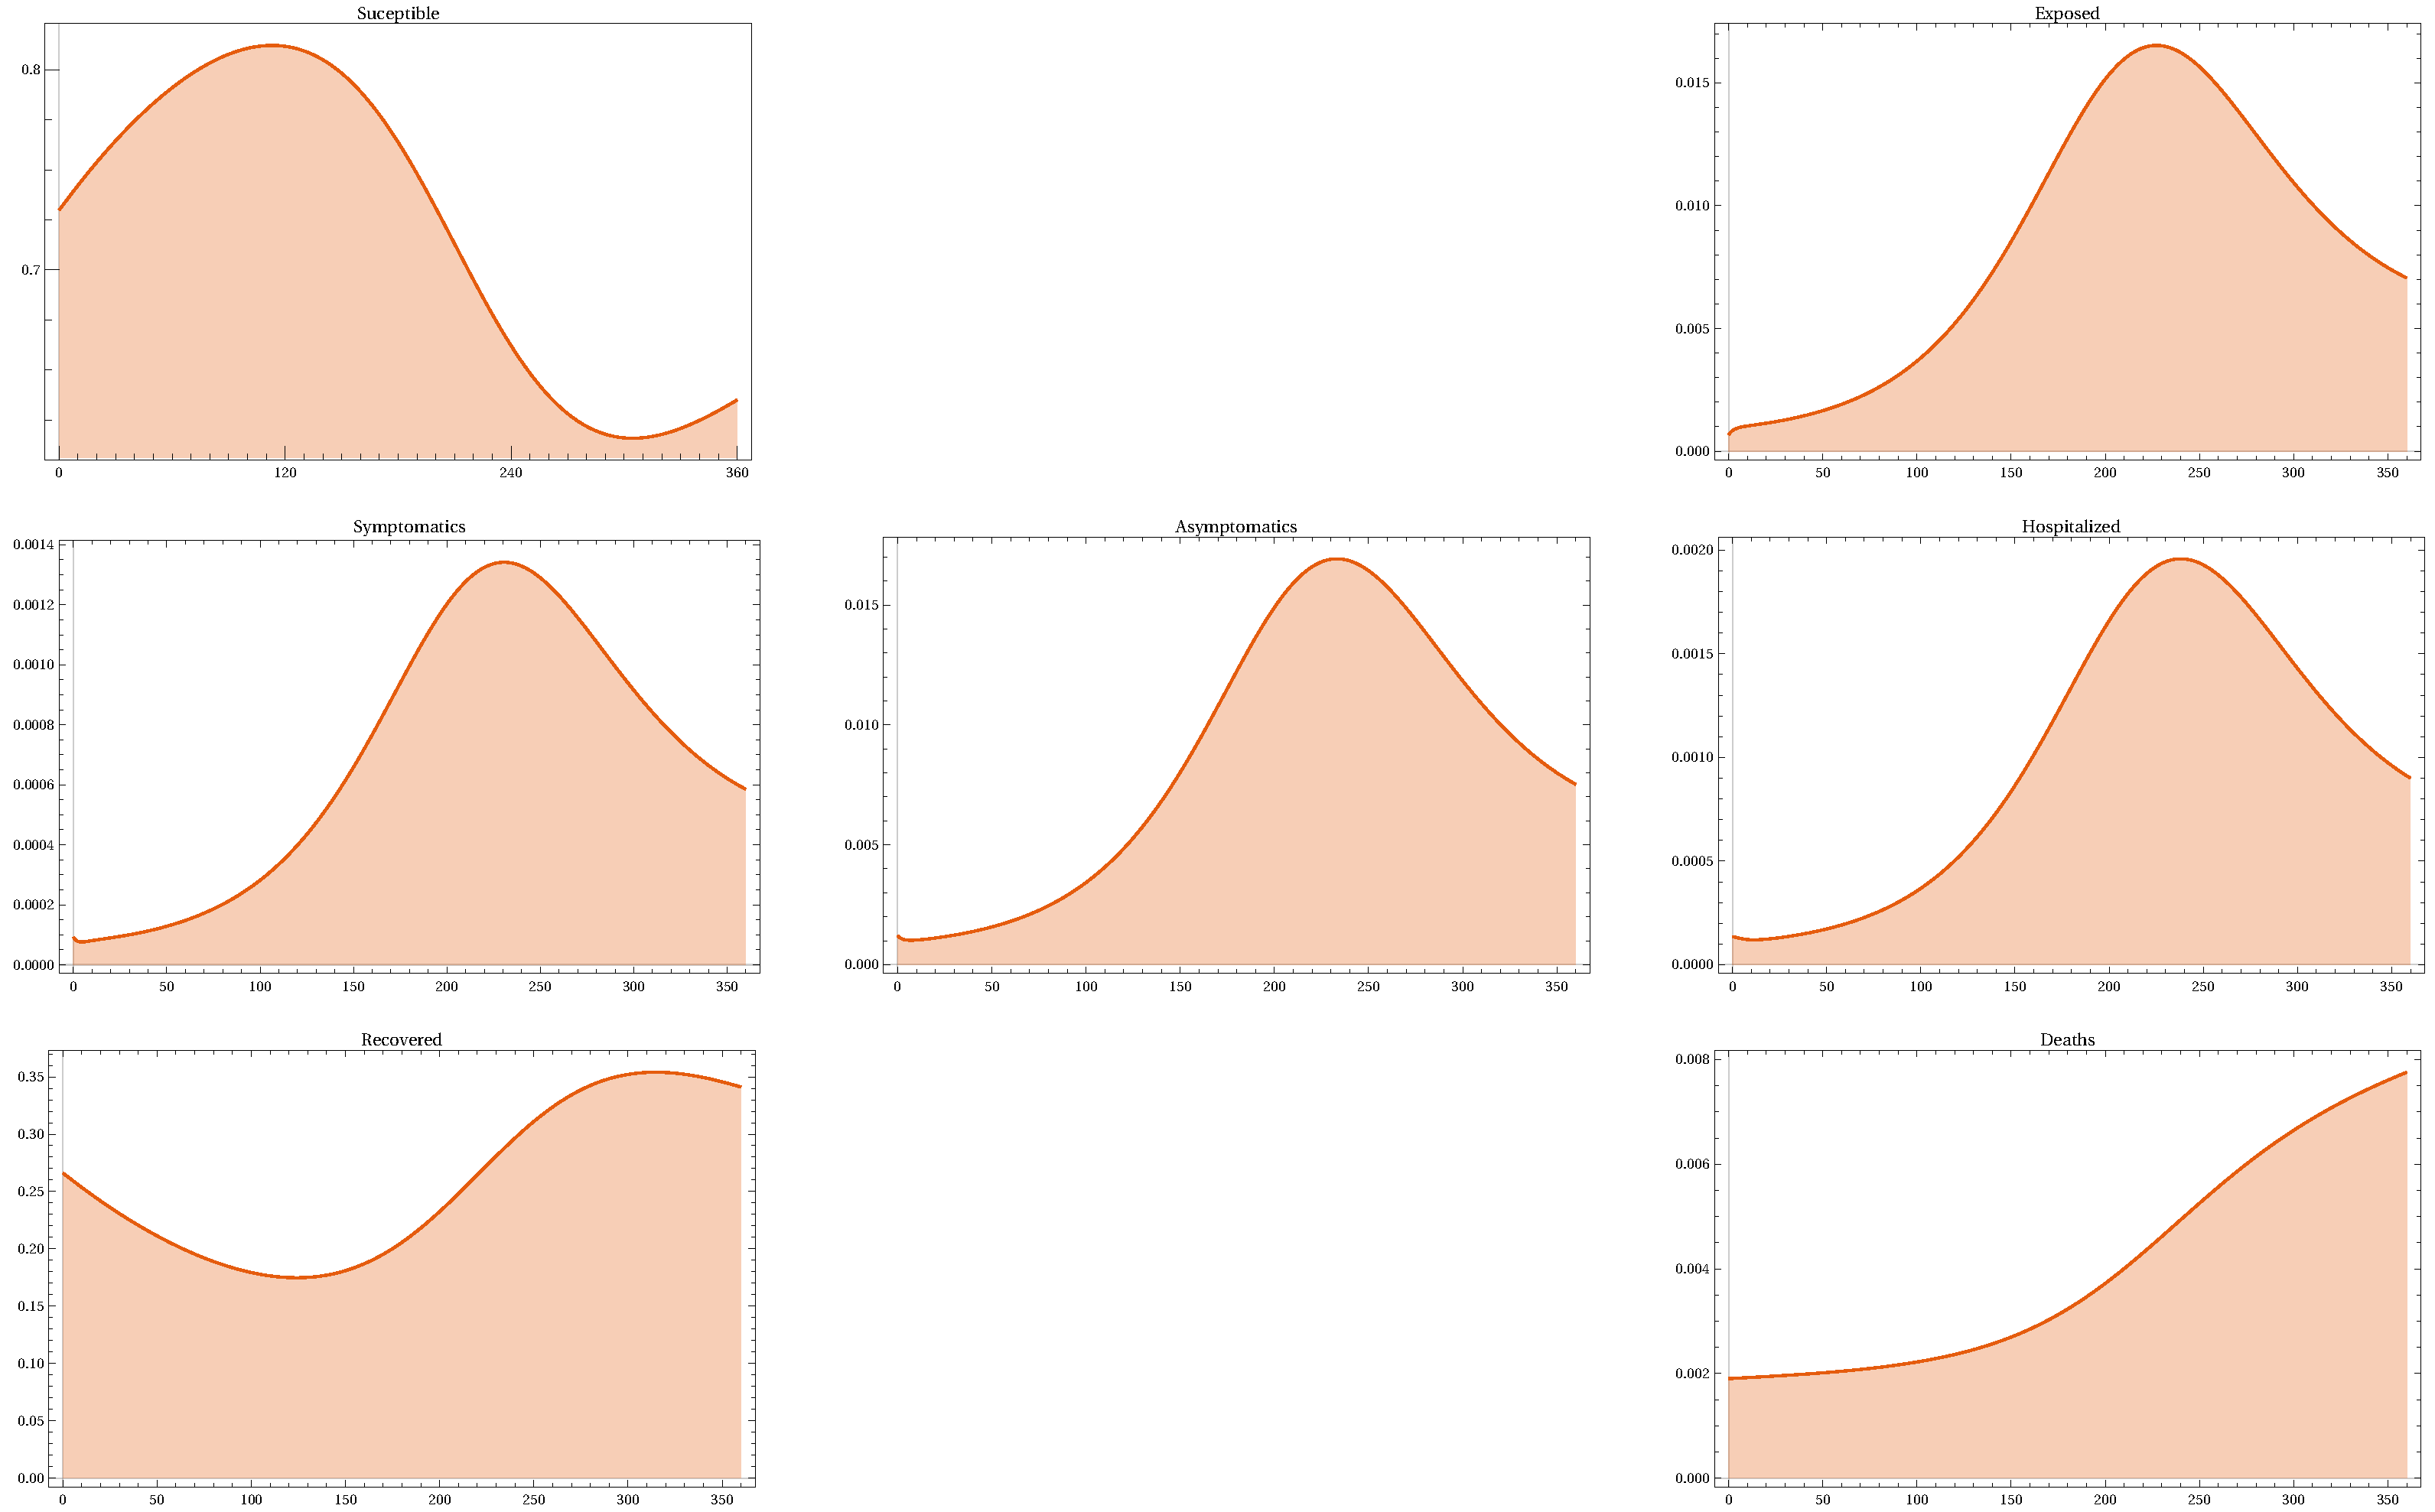
\includegraphics[scale=0.25,
        keepaspectratio]{no_contraled_dynamics}
    \end{center}
    \caption{
        Spreed dynamics of COVID-19 according to model in
        \Cref{eqn:base_dynamics}.
    }
    \label{fig:base_dynamics}
\end{figure}

    We display in \Cref{fig:base_dynamics} a typical evolution of this COVID-19 spreed dynamics.
\Cref{tbl:dynamics_base_parameters} encloses notation and reference values.
%
\begin{table*}[h!]
	\centering
	\begin{tabular}{>{\centering}%
        p{0.2\textwidth}%
        p{0.4\textwidth}
    }
    \toprule
		\textbf{Parameter} & \textbf{Description}
  	\\
  	\midrule
		$\mu$ &
			Death rate
		\\
        $\beta_S$ &
        	Infection rate between susceptible and symptomatic infected
		\\
        $\beta_A$ &
        	Infection rate between susceptible and asymptomatic infected
		\\
        $\lambda_V$ &
        	Vaccination rate
		\\
        $\delta_{V}^{-1}$ &
        Vaccine-induced immunity
		\\
        $\varepsilon$ &
        	Vaccine efficacy
		\\
        $\kappa^{-1}$ &
        	Average incubation time
        \\
		$p$ &
			New asymptomatic generation proportion
		\\
	    $\theta$ &
        	Proportion of suceptible individuals under lockdown
        \\
        $\gamma_{S}^{-1}$ &
        	Average time of symptomatic recovery
        \\
		$\gamma_{A}^{-1}$ &
			Recovery average time of asymptomatic individuals
		\\
		$\gamma_{H}^{-1}$ &
			Recovery average time by hospitalization
		\\
        $\delta_{R}^{-1}$ &
        	Natural immunity
  		\\
  		$\delta_{H}$ &
        	Infected symptomatic hospitalization rate
  		\\
  	\bottomrule
	\end{tabular}
		\caption{
			Parameters definition of model in
			\Cref{eqn:base_dynamics}.}
    \label{tbl:dynamics_base_parameters}
\end{table*}
%
\begin{figure*}[htb]
    \centering
    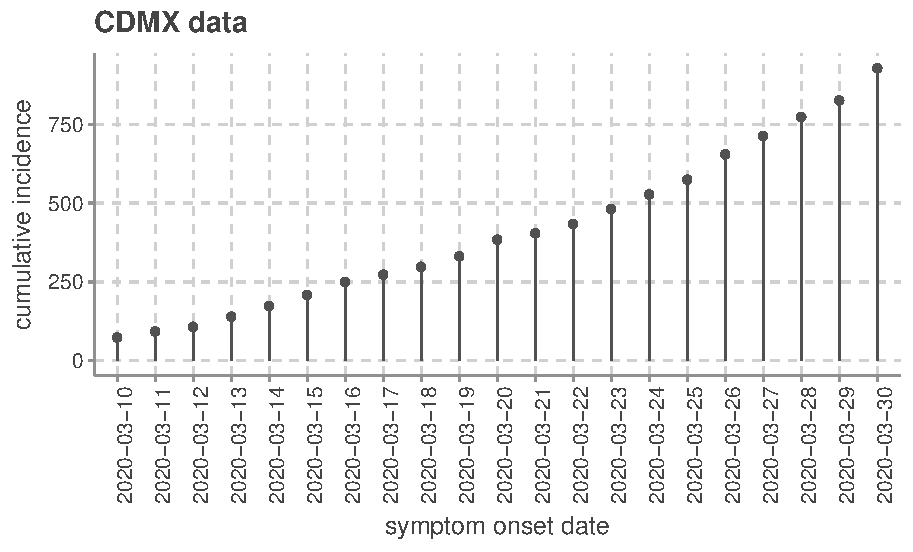
\includegraphics[scale=0.8, keepaspectratio]{Figures/cdmx_input_data}
    \caption{%
        Cumulative new symptomatic and confirmed COVID19 reported cases from
        Ciudad de Mexico and Valle de Mexico
        \cite{cdmxDATA} between March, 10, to March 30 of
        2020.
        \href{https://plotly.com/~AdrianSalcedo/48/}{%
		https://plotly.com/~AdrianSalcedo/48/}
	}
    \label{fig:data_CDMX}
\end{figure*}
%
